\documentclass[conference]{IEEEtran}

\usepackage{cite}
\usepackage{amsmath}
\usepackage{graphicx}
\usepackage{url}

\begin{document}

\title{A Fly Genome for Robots: 256 Neurons on Arduino and Raspberry Pi}

\author{\IEEEauthorblockN{Robofly Project}}

\maketitle

\begin{abstract}
We describe a representation of the fly's sensorimotor genome, compiled so a robot can run it.
The genome is the published escape and motor program: eight looming bins, LPLC2, LC4, the giant fiber, a PSI, thrust, and the motor pairs.
It is 256 leaky integrate-and-fire neurons and 670 synapses, and it steps every 50\,ms.
Pitch follows the hunter, so the nose and the height rise and fall together inside a mid band.
The same tick runs in a Python simulator, in the WebAssembly explorer, and as firmware for a Raspberry Pi or an Arduino-class board.
The circuits below are a reference design for a machine that already has an ordinary limiter around its motors.
\end{abstract}

\section{Introduction}
A fly leaves a looming object with a short, directional takeoff, and it climbs as it turns.
The cells that detect the loom, and the giant fiber that releases the jump, are known in enough detail to compile that program into a controller \cite{klapoetke2017,vonreyn2014}.
The adult wiring diagram is public \cite{dorkenwald2024,scheffer2020}.
This paper takes the escape path and the motor pairs from that map and compiles them into a fixed graph of 256 neurons that finishes inside a 50\,ms frame.
The name, and the aim of a fly-scale robot, take inspiration from the University of Washington RoboFly of Chukewad, James, Singh, and Fuller \cite{chukewad2021}.

A Raspberry Pi runs the graph in floating point.
An Arduino-class board runs the same graph in fixed point.
The explorer on the project site is that controller, playing in a browser, so the behavior can be watched before anyone wires a motor.
The sections below give the membrane update, the motor rate, the looming weights, the pitch and lift that move the body, the wall mix, and the pin maps.

Open robot platforms and neuromorphic chips are the neighbors of this design.
OpenBot and Duckietown showed that a documented, inexpensive platform is a research object of its own \cite{muller2021,paull2017}.
Loihi showed what a manycore neuromorphic processor is for \cite{davies2018}.
The machine here is a genome small enough to copy onto boards people already have.

\section{Related work}
The hemibrain reconstructed a large part of the adult central brain \cite{scheffer2020}.
FlyWire then published a whole adult brain, 139{,}255 neurons and about 54.5 million chemical synapses \cite{dorkenwald2024}.
That map is the source of the programs compiled here.
The live tick keeps the looming detectors, the giant-fiber order, and the motor pairs, in a graph that finishes inside one frame.

Looming detection in the fly optic lobe is carried by LPLC2 cells that respond to radial expansion \cite{klapoetke2017}.
The giant fiber releases a stereotyped jump and flight start, and the timing of visual spikes selects that action \cite{vonreyn2014}.
Descending neurons carry the decision from the brain toward the motor plants \cite{namiki2018}.
The controller keeps the order of that chain and a direction-specific turn.

Open platforms are the other neighbor.
OpenBot turns a phone into a driving robot and reports the hardware, the software, and the measured behavior \cite{muller2021}.
Duckietown does the same for a city of small cars \cite{paull2017}.
We follow that pattern: one graph, two boards, and a public explorer.
The measurements are taken in the simulator and in that explorer.

\section{The membrane}
One step is the same in every implementation.
The world, or the pins that stand in for it, becomes a sensory current \(d_i\).
A cell that is free of its refractory period updates
\begin{equation}
v_i \leftarrow 0.92\, v_i + d_i + \sum_j s_j w_{ji},
\label{eq:lif}
\end{equation}
where \(s_j \in \{0,1\}\) is the spike of the presynaptic cell on the previous tick and \(w_{ji}\) is the stored weight.
A cell still in refractory is held at \(v_i = 0\).
The cell spikes when \(v_i \ge 1\).
The spike clears the voltage and sets a refractory period of two ticks.
Figure~\ref{fig:chip} is that tick: sensors into the membranes, spikes through the synapse memory, motor accumulators, then the body.

\begin{figure*}[t]
\centering
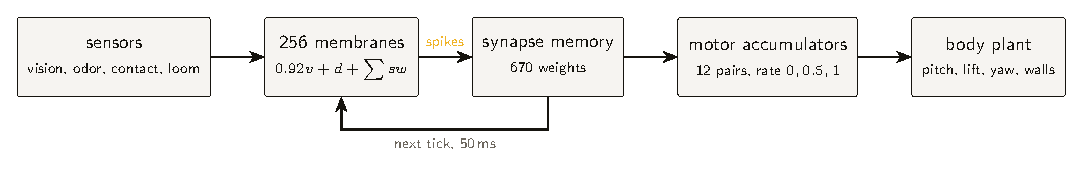
\includegraphics[width=0.98\textwidth]{figures/chip.pdf}
\caption{One 50\,ms tick. Sensory current enters 256 membranes. Spikes address the 670 stored weights on the next tick. Twelve motor pairs accumulate into the body plant.}
\label{fig:chip}
\end{figure*}

The twelve motor commands are pairs.
The rate of a pair is the mean of its two spike bits,
\begin{equation}
r = \tfrac{1}{2}(s_a + s_b),
\label{eq:rate}
\end{equation}
so a command is 0, 0.5, or 1.
The body plant turns those rates into thrust, yaw, pitch, and lift, then the pose advances by one 50\,ms step.

The default graph has 256 neurons and 670 synapses.
Vision occupies cells 0--63, odor 64--79, contact 80--87, and looming 88--95.
The last 24 cells are the twelve motor pairs.
The cells between are interneurons.
The wired programs carry the live behavior: the escape path, the direct sensor-to-motor edges, and the body plant.
Figure~\ref{fig:populations} is that layout.

\begin{figure*}[t]
\centering
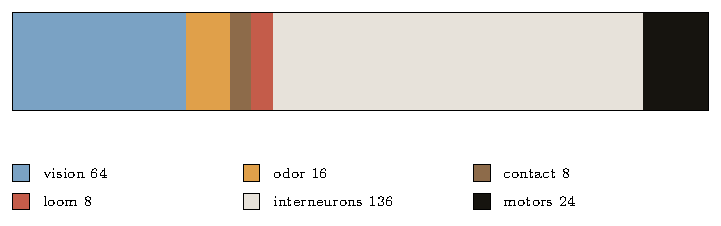
\includegraphics[width=0.86\textwidth]{figures/populations.pdf}
\caption{The 256-cell genome. Vision, odor, contact, and looming are the sensory populations. Twelve motor pairs occupy the last 24 cells.}
\label{fig:populations}
\end{figure*}

The Python simulator, the WebAssembly module in the explorer, and the firmware take the same step.
A food-search trace of 40 ticks is the parity check between Python and WebAssembly.

\section{The escape chain}
Looming is divided into eight non-overlapping \(45^\circ\) bins in the body frame.
The center of bin \(k\) is
\begin{equation}
\theta_k = -\pi + \left(k + \tfrac{1}{2}\right)\frac{\pi}{4}.
\label{eq:bins}
\end{equation}
Ahead is the shared edge of bins 3 and 4.
Positive bearing is left.
Each bin drives one LPLC2-like cell.
Those cells also drive one LC4-like cell.
LPLC2 and LC4 both drive a giant fiber.
The giant fiber drives an escape pair, the jump motor program, and a PSI.
The PSI drives the thrust pair, the wing-depressor program.
Each LPLC2 also drives the yaw pair on the opposite side, so the body turns away from the loom.
The forward and side bins use chain weight 1.15.
The two rear bins, 0 and 7, use
\begin{equation}
w_{\mathrm{rear}} = 1.15\,|\sin \theta_k|\,0.4,
\label{eq:rear}
\end{equation}
which leaves the heading when the threat is already behind.
Figure~\ref{fig:chain} is that order, and Figure~\ref{fig:rose} is the eight bins.

\begin{figure*}[t]
\centering
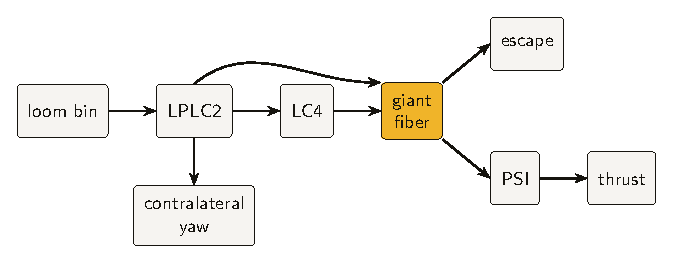
\includegraphics[width=0.92\textwidth]{figures/escape_chain.pdf}
\caption{The escape genome. A loom bin drives LPLC2, LC4, the giant fiber, escape, and thrust through the PSI. LPLC2 also drives the yaw pair that turns away.}
\label{fig:chain}
\end{figure*}

\begin{figure*}[t]
\centering
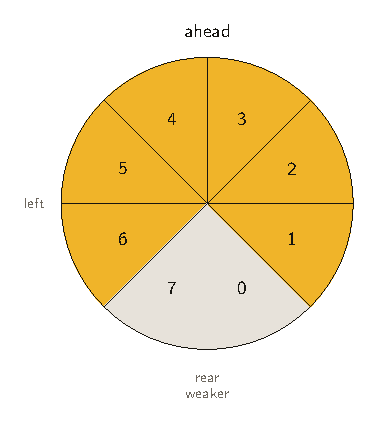
\includegraphics[width=0.62\textwidth]{figures/loom_rose.pdf}
\caption{Eight body-frame looming bins. Ahead is up and left is positive. Bins 0 and 7, behind the fly, use the weaker yaw weight.}
\label{fig:rose}
\end{figure*}

A yaw command is latched for two ticks, because the looming cells spike one tick before the escape motor.
Escape is then held for six ticks, with a forward dash of 0.034\,m per tick, and a saccade cooldown of seven ticks keeps the next turn for a later loom.
This chain uses the looming population and the yaw pairs already in the 256.

\section{Pitch, lift, and walls}
Feed, groom, walk, land, and rest are direct wires from contact or from a command sensor to the matching motor.
Odor on the left drives yaw one way and a share of thrust.
Odor on the right drives the other yaw.
Vision on one side drives the opposite yaw.
A threat inside the loom range and below the body drives the pitch-up pair.
With horizontal gap \(h\) and height gap \(\Delta z\), the drive on that pair is
\begin{equation}
d_{\mathrm{up}} = 1.4\, \sigma \max\!\left(0, -\sin \operatorname{atan2}(\Delta z, h)\right),
\label{eq:below}
\end{equation}
where \(\sigma\) is the loom strength.
These edges are the rest of the motor genome, stored as the same kind of synapse as the escape chain.

With a hunter inside the loom range, the held height follows that hunter and eases back from the top of the band,
\begin{equation}
\begin{aligned}
q &= \operatorname{clamp}(z_{h} + 0.55,\; 0.9,\; 1.7), \\
h^{\star} &= \min\!\big(q,\; 0.5q + 0.575\big), \\
g &= h^{\star} - z.
\end{aligned}
\label{eq:held}
\end{equation}
The pitch pair is smoothed into a climb bias \(b \leftarrow 0.85b + 0.15 r_{\mathrm{up}}\).
The nose eases toward the gap, and the bias still adds nose-up while the hunter is below the fly,
\begin{equation}
\begin{aligned}
\alpha &= \operatorname{clamp}(2.4g + 0.06b_{\downarrow},\,-0.35,\,0.4), \\
\phi &\leftarrow 0.8\,\phi + 0.2(\alpha - 0.45\, r_{\mathrm{land}}).
\end{aligned}
\label{eq:pitch}
\end{equation}
where \(b_{\downarrow}\) is \(b\) while the hunter is below and 0 otherwise.
While the fly is off the pad, lift is the damped vertical speed plus a climb from the nose and from the gap, clamped between \(-0.02\) and \(0.028\),
\begin{equation}
\ell = \operatorname{clamp}\!\big(-0.28\, v_z + \sin\phi \cdot u_{+} + 0.018\,\operatorname{clamp}(g,-1,1)\big),
\label{eq:lift}
\end{equation}
where \(u_{+}\) is the forward speed when it is positive.
Nose-up climbs.
Nose-down descends.
With no hunter in range the gap is zero, the nose eases back to level, and the height already reached is held.
Landing is a steady descent of 0.045 until the floor, and escape clears the landing hold so a pad under a fleeing fly leaves the body in the air.
Figure~\ref{fig:pitch} is a yard trace from the Python plant, seed 1701.
The nose dips, then rises, and the height falls from 1.2\,m before climbing into the band and holding there.

\begin{figure*}[t]
\centering
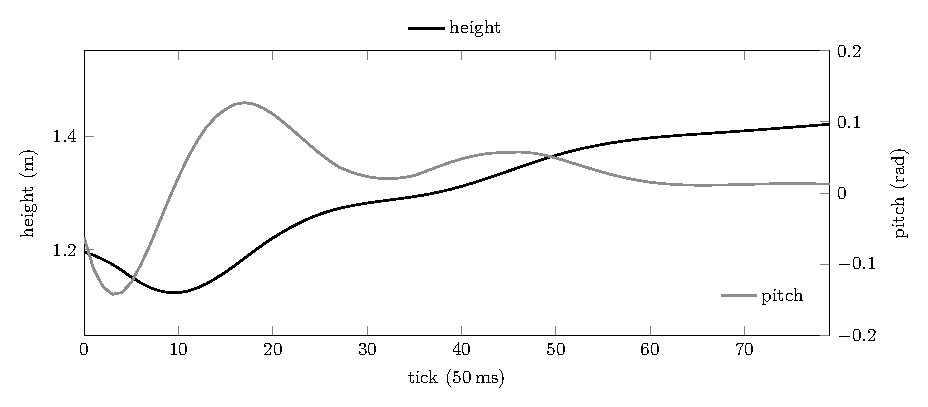
\includegraphics[width=0.92\textwidth]{figures/pitch_trace.pdf}
\caption{Pitch and height on the yard, one point per 50\,ms tick. The nose and the height fall, then rise, and the body holds the band above the hunter.}
\label{fig:pitch}
\end{figure*}

Odor falls as \(\exp(-d / 12)\), so a food about ten meters away still moves thrust and yaw.
Looming reaches 16\,m.
Vision stays at 2.3\,m, so a nearby wall stays a clearance problem for the body plant.

The chip decides escape and the turn.
While a threat is present and the fly is airborne, forward speed is held at a cruise of at least 0.016.
With clearance \(c\) ahead and a wall-avoid command \(a\), the yaw command is replaced when the nose is close and mixed when it is only near,
\begin{equation}
\psi \leftarrow
\begin{cases}
a & c < 0.55,\\
0.55\,\psi + a & c < 1.2.
\end{cases}
\label{eq:wall}
\end{equation}
Speed aimed into a wall is capped from that same clearance.
A hunter that comes within its radius plus 0.22\,m sends the fly back to the scene start.
The next 30 ticks are a shield, so the fly can leave.

\section{Reference circuits}
Both boards see a range and a bearing, and both emit thrust, two yaw directions, and escape.
Range and bearing carry the looming direction the explorer computes from a predator in the room.

On a Raspberry Pi the firmware is the Python tick.
The Pi has the memory and the floating-point unit to keep the same arithmetic as the simulator.
The map is GPIO 17 for loom range, GPIO 27 for bearing, GPIO 12 and 13 and 18 as PWM for thrust and the two yaw directions, and GPIO 22 as a digital escape line.

On an Arduino-class board the same 256 cells and 670 synapses are a fixed-point loop.
Decay, threshold, and the synapse weights fit in 16-bit or 32-bit integers.
A few hundred multiply-adds are a short inner loop.
A 50\,ms frame fits a common AVR part and an ESP32-class part.
The pins are A0 for range, A1 for bearing, D5, D6, and D9 as PWM for thrust and yaw, and D3 as digital escape.

The repository also emits SystemVerilog for the same graph.
That core checks that the spike rule can be written as hardware.
The board firmware is the tick in the previous paragraphs.

\section{The explorer as the testbed}
The measurements in this project come from the deterministic simulator and from the explorer that runs the WebAssembly twin.
The scenes used as the bar are a food trail that is eaten, an escape that opens a gap and turns away, a cruise that holds while a hunter is present, a climb whose drop from the peak stays under 0.35\,m, a wall clearance of 0.7\,m, a gate the fly goes around, a landing onto a pad, a quiet room that stays put, and a yard that stays inside its court.
A catch returns the body to the start, which is checked by placing the hunter on the fly.

Figure~\ref{fig:trace} is the first 80 ticks of the loom scene, recorded from the Python plant with seed 1701.
On tick 3 the yaw-right pair fires and the body turns away.
From tick 4, escape and thrust alternate as the refractory period hands the spike from the escape pair to the thrust pair.
The same trace is what the explorer plays.

\begin{figure*}[t]
\centering
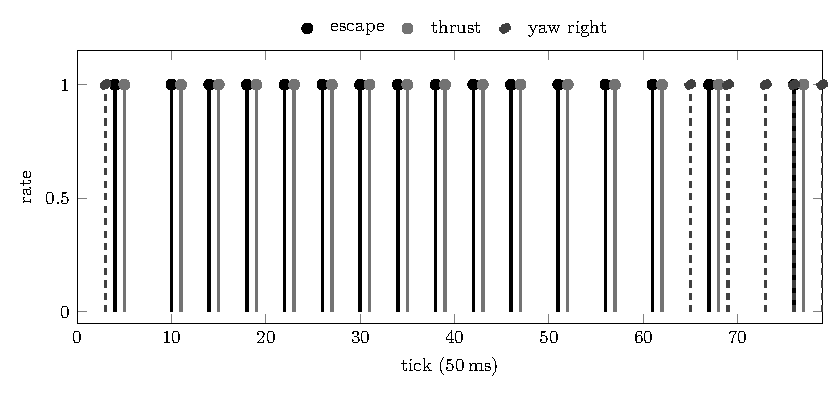
\includegraphics[width=0.92\textwidth]{figures/escape_trace.pdf}
\caption{Motor rates from the loom scene. Each tick is 50\,ms. Yaw right fires as the fly turns off the threat, then escape and thrust alternate for the dash.}
\label{fig:trace}
\end{figure*}

The explorer is the running copy of the tick.
The whitepaper on the site is the short account.
This preprint is the full account of the controller above.

\section{Conclusion}
A fly escape path, compiled with the motor pairs into 256 neurons, runs every 50\,ms on an Arduino or a Raspberry Pi.
The membrane is \eqref{eq:lif}, the motor rate is \eqref{eq:rate}, and the looming bins are \eqref{eq:bins} with the rear weight \eqref{eq:rear}.
The nose follows \eqref{eq:pitch} and the climb follows \eqref{eq:lift}, with the wall mix \eqref{eq:wall} beside them.
The explorer is the running copy of the tick.
The circuits are how that copy leaves the browser.

\bibliographystyle{IEEEtran}
\bibliography{refs}

\end{document}
